\documentclass[11pt,a4paper]{article}
\usepackage[T1]{fontenc}
\usepackage[utf8]{inputenc}
\usepackage{lmodern,microtype}
\usepackage[margin=23mm]{geometry}
\usepackage{amsmath,amssymb,booktabs,array,graphicx,siunitx,xurl}
\usepackage[numbers,sort&compress]{natbib}
\usepackage[colorlinks=true,linkcolor=blue!50!black,citecolor=blue!50!black,urlcolor=blue!50!black]{hyperref}
\usepackage{xcolor,placeins}
\graphicspath{{figures/}}
\newcommand{\dd}{\mathrm{d}}
\newcommand{\code}[1]{\path{#1}}
\newcommand{\sinc}{\operatorname{sinc}}
\newcommand{\CD}{C_D}
\newcommand{\Cf}{C_f}
\newcommand{\Tcds}{T_{\rm CDS}}
\newcommand{\Vref}{V_{\rm REF}}
\newcommand{\Voff}{V_{\rm OFF}}
\setlength{\parindent}{0pt}
\setlength{\parskip}{5pt plus 1pt}
\setlength{\emergencystretch}{3em}
\title{NAUSICAA v2\\[4pt]\large The charge-sensitive amplifier: noise, filtering and architecture}
\author{V. Herrero \and J. Garc\'ia (J.J. Gómez-Cadenas as student and scribe)}
\date{13 November 2026}
\begin{document}
\maketitle
\begin{abstract}
This note analyses the charge-sensitive amplifier for the NAUSICAA ion
readout. It derives the transfer function of the amplifier, the three sources of
electronic noise and
their expression as an equivalent charge at the pad, the effect of integrating
over a frame and of subtracting consecutive frames, and the charge
bookkeeping of a two-capacitor architecture that performs that subtraction in
the analogue domain. It then analyses a cascode amplifier with source degeneration, the
bandwidth and stability constraints of a real amplifier, and the role of the
pad capacitance. The last section compares the reset architecture with the
continuous-discharge amplifier simulated and calibrated in this repository.
\end{abstract}
\tableofcontents

% ----------------------------------------------------------------------
\section{Notation and scope}
\label{sec:notation}
%
The analysis uses one set of symbols throughout.
%
\begin{itemize}
\item $\CD$: capacitance of the pad and its connection to the amplifier
  input, in farad, between \SIlist{1;5}{pF} for the TopMetal pad. Where the amplifier's
  own input capacitance matters it is included in $\CD$.
\item $\Cf$: feedback capacitance. The present NAUSICAA circuit uses
  \SI{3}{fF}.
\item $A$: open-loop voltage gain of the amplifier, dimensionless and
  negative in sign convention, written $-A$ with $A>0$.
\item $e_n^2(f)$: one-sided spectral density of the voltage noise referred to
  the amplifier input, in \si{V^2/Hz}. It has a white part $e_t^2$ (thermal)
  and a flicker part $A_f/f$. The corner frequency $f_c=A_f/e_t^2$ is where
  the two are equal.
\item $i_R^2=4kT_{\rm K}/R_f$: spectral density of the current noise of a feedback
  resistor $R_f$ at temperature $T_{\rm K}$, in \si{A^2/Hz}; $k$ is
  Boltzmann's constant and $4kT_{\rm K}=\SI{1.66e-20}{J}$ at \SI{300}{K}.
\item $T$: length of the integration window, one readout frame. The
  NAUSICAA productions use \SIlist{20;30;40}{ms}.
\item $\Tcds$: interval between the two samples that are subtracted. For
  consecutive frames $\Tcds=T$.
\item ENC: equivalent noise charge, the root-mean-square charge at the pad
  that would produce the observed output noise, expressed in electrons
  ($e=\SI{1.602e-19}{C}$).
\end{itemize}
%
Each section states a circuit or an operation, derives its result, and
says what it means for NAUSICAA. Key results are boxed. The standard
references for this material are Spieler~\cite{Spieler2005},
Radeka~\cite{Radeka1988} and Gatti and Manfredi~\cite{GattiManfredi1986}.
Correlated double sampling comes from CCD readout~\cite{Janesick2001}.

% ----------------------------------------------------------------------
\section{The charge-sensitive amplifier}
\label{sec:csa}
%
\begin{figure}[htbp]\centering
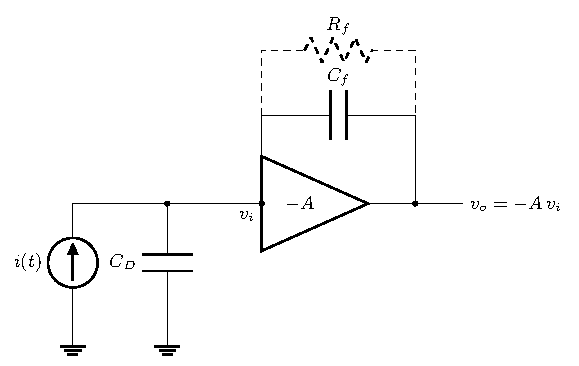
\includegraphics[width=.55\linewidth]{nausicaa_vh_csa.pdf}
\caption{The pad is a current source $i(t)$ in parallel with its capacitance
$\CD$. The amplifier has gain $-A$ and feedback capacitance $\Cf$. The dashed
resistor $R_f$ is present in a continuous-discharge amplifier and absent in a
reset amplifier.}
\label{fig:csa}
\end{figure}
The ions arriving at the pad induce a current $i(t)$. Figure~\ref{fig:csa}
shows the circuit. Write $v_i$ for the voltage at the input node and
$v_o=-Av_i$ for the output. Charge conservation implies 
that the current $i$ delivered by the pad is shared by the two capacitors:
%
\begin{equation}
 i(t) = i_{\CD}(t) + i_{\Cf}(t).
\end{equation}
%

The current through a capacitor is the rate of change of the charge on it,
$i_C=C\,\dd v_C/\dd t$, where $v_C$ is the voltage across its plates. The
voltage across $\CD$ is $v_i$; the voltage across $\Cf$ is $v_i-v_o$. Hence
%
\begin{equation}
 i(t) = \CD\,\frac{\dd v_i}{\dd t} + \Cf\,\frac{\dd (v_i-v_o)}{\dd t}.
\label{eq:kcltime}
\end{equation}
%

In the Laplace domain\footnote{The Laplace transform of a function of time
$x(t)$ is
%
\[
 X(s) = \int_0^\infty x(t)\,e^{-st}\,\dd t ,
\]
%
where $s$ is a complex variable. The transform of a derivative follows by
integrating by parts:
%
\[
 \int_0^\infty \frac{\dd x}{\dd t}\,e^{-st}\,\dd t
 = \Big[x(t)\,e^{-st}\Big]_0^\infty + s\int_0^\infty x(t)\,e^{-st}\,\dd t
 = s\,X(s) - x(0).
\]
%
The boundary term at infinity vanishes for any signal that grows slower than
$e^{st}$. The term $x(0)$ is the initial value; for the response to a signal
that starts from rest it is zero, and for noise it only shifts the mean.
With that convention a derivative in time is a multiplication by $s$. Each
term of Eq.~\eqref{eq:kcltime} transforms separately, since the transform is
linear and the capacitances are constants:
$\CD\,\dd v_i/\dd t\to s\CD V_i(s)$,
$\Cf\,\dd(v_i-v_o)/\dd t\to s\Cf[V_i(s)-V_o(s)]$ and $i(t)\to I(s)$.}
Eq.~\eqref{eq:kcltime} becomes
%
\begin{equation}
 I(s) = s\,\CD\,V_i(s) + s\,\Cf\,\big[V_i(s)-V_o(s)\big],
\label{eq:kcls}
\end{equation}
%
where $s$ is the Laplace variable.\footnote{For a signal that is a steady
sinusoid of angular frequency $\omega$, every voltage and current can be
written as a complex amplitude times $e^{j\omega t}$, for example
$v_i(t)=\mathrm{Re}\,[V_i\,e^{j\omega t}]$, with
$e^{j\omega t}=\cos\omega t+j\sin\omega t$. Then
$\dd(V_i e^{j\omega t})/\dd t = j\omega\,V_i\,e^{j\omega t}$:
differentiation multiplies the amplitude by $j\omega$, and the common factor
$e^{j\omega t}$ cancels from every term of the equation. The Laplace variable
restricted to the imaginary axis, $s=j\omega$, therefore describes the
response to sinusoids, which is the frequency response. A general signal is a
superposition of sinusoids, so the frequency response determines the
response to anything. The magnitude $|V_i|$ is the amplitude of the sinusoid
and the argument of $V_i$ its phase.}
The voltage across the feedback capacitor is the difference between its
two plates. One plate is the input node, at $v_i$. The other is the output,
and the amplifier inverts: $v_o=-Av_i$. When the input rises by $v_i$ the
output falls by $Av_i$, so the two plates move in opposite directions and the
capacitor sees the sum of the two excursions,
%
\begin{equation}
 v_i - v_o = v_i + A\,v_i = (1+A)\,v_i .
\label{eq:miller}
\end{equation}
%
The capacitor therefore draws $1+A$ times the current that a grounded
capacitor of the same value would draw at the same input voltage\footnote{This is
the Miller effect: seen from the input node, $\Cf$ behaves as a capacitance
$(1+A)\Cf$ to ground.}. Substituting Eq.~\eqref{eq:miller} in
Eq.~\eqref{eq:kcls}, and writing the transforms in lowercase from here
on,\footnote{In
Eq.~\eqref{eq:kcls}, $i(t)$ is the pad current and $I(s)$ its transform.
Circuit analysis usually drops the uppercase and uses one symbol for both,
because the equations are almost always written in the transformed domain.
The rest of this note follows that practice: a symbol written with the
argument $t$, such as $i(t)$ or $v_o(t)$, is a function of time; the same
symbol written without argument or together with $s$, as in $i=s\CD v_i$, is
the transform.}
%
\begin{equation}
 i = s\CD\,v_i + s\Cf\,(v_i-v_o) = s\,v_i\,[\CD+(1+A)\Cf].
\label{eq:kcl}
\end{equation}
%

Equation~\eqref{eq:kcl} gives the input voltage produced by the pad
current, $v_i = i/\{s[\CD+(1+A)\Cf]\}$. The output is $-A$ times that:
%
\begin{equation}
 v_o = -A\,v_i = -\frac{A}{s\,[\CD+(1+A)\Cf]}\; i .
\label{eq:vofull}
\end{equation}
%
For a large gain, $A\Cf\gg\CD$ and $A\gg1$, the bracket is $A\Cf$ and the
gain cancels:
%
\begin{equation}
 v_o \;\xrightarrow{\;A\Cf\gg\CD\;}\; -\frac{1}{s\Cf}\; i .
\label{eq:vo}
\end{equation}
%
Division by $s$ is integration in time. For a large gain the output is
%
\begin{equation}
 \boxed{\;v_o(t) = -\frac{1}{\Cf}\int_0^t i(t')\,\dd t' = -\frac{Q(t)}{\Cf}\;}
\label{eq:qoverc}
\end{equation}
%
the charge collected so far divided by the feedback capacitance. 

Three
properties follow from Eqs.~\eqref{eq:kcl} to \eqref{eq:vo}.
%
\begin{itemize}
\item The input node is a virtual ground: $v_i=-v_o/A$ is small, so the pad
  stays at a fixed potential while charge flows into the amplifier.
\item The output does not depend on $\CD$ as long as $A\Cf\gg\CD$. The gain
  is set by one capacitor  ---thus the name,  charge sensitive amplifier---.
\item Part of the charge stays on the pad. The input node is connected to
  two capacitances charged to the same voltage $v_i$: $\CD$ to ground and,
  through the Miller effect, $(1+A)\Cf$ to the output. Each takes charge in
  proportion to its capacitance,
%
  \begin{equation}
   Q_D = \CD\,v_i, \qquad Q_f = (1+A)\,\Cf\,v_i, \qquad Q = Q_D + Q_f ,
  \end{equation}
%
  and only $Q_f$ reaches the output. The fraction left on the pad is
%
  \begin{equation}
   \frac{Q_D}{Q} = \frac{\CD}{\CD+(1+A)\Cf} .
  \label{eq:sharing}
  \end{equation}
%
  With $\Cf=\SI{3}{fF}$ and $A=1000$ the Miller capacitance is
  \SI{3.0}{pF}, comparable to a \SI{1.25}{pF} pad, and
  \SI{29}{\percent} of the charge never reaches the output; for $A=10^4$
  the fraction is \SI{4}{\percent}. Either the open-loop gain is made large
  enough for this fraction to be negligible, or the calibration measures the
  actual output per ion and absorbs it.
\end{itemize}
%

The feedback resistor $R_f$ of Fig.~\ref{fig:csa} lets the collected charge
leak away with the time constant $\tau_f=R_f\Cf$, so that the output returns
to its resting value and the amplifier never saturates. The present NAUSICAA
amplifier uses a transistor for this purpose, with a measured
small-signal decay time of \SI{19.5}{s}. This note proposes the
alternative: remove the resistor and reset the amplifier with a switch,
using the two-capacitor architecture of Section~\ref{sec:swap}. 
%The choice
%between the two decides the noise, as the next sections show.

% ----------------------------------------------------------------------
\section{Sources of noise and their equivalent charge}
\label{sec:noise}
%
\begin{figure}[htbp]\centering
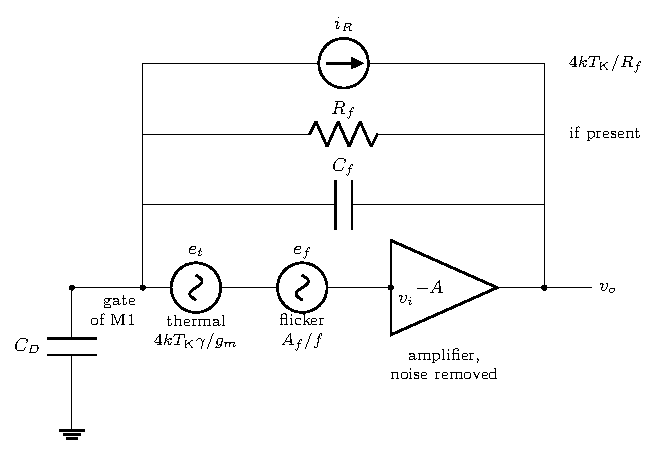
\includegraphics[width=.5\linewidth]{nausicaa_vh_noise.pdf}
\caption{Noise model. The input transistor contributes two voltage sources
referred to its gate, thermal $e_t$ and flicker $e_f$; they are independent,
so their mean squares add, $e_n^2=e_t^2+e_f^2$. They sit between the gate of M1,
where the pad and the feedback branch meet, and the rest of the amplifier,
which has no noise left once the sources are placed in front of it and whose
input $v_i$ is the virtual ground. A feedback resistor, if present, injects its
current noise $i_R$ directly into the gate node, in parallel with $\Cf$.}
\label{fig:noise}
\end{figure}
The amplifier $A$ of Fig.~\ref{fig:csa} is a transistor circuit. 
Fig.~\ref{fig:cascode} shows a possible implementation (a cascode). The noise of
the circuit is dominated by the input transistor (M1 in the figure)\footnote{The
pad is directly connected to M1 gate and the noise of all the other transistors
referred to that gate is suppressed by their
gain.}.

The noise of M1 is represented by voltage sources in series with its gate,
chosen to produce the same drain-current fluctuation as the transistor
itself (the companion note on electronic noise~\cite{GomezCadenas2026noise}
constructs them for the thermal part).
What remains behind the sources is the amplifier with its noise removed,
whose input is still the virtual ground. The gate of M1 is thus split in
two: the physical gate node, where the pad and the feedback branch connect,
and the input of the noiseless amplifier, with the noise sources between
them.

Fig.~\ref{fig:noise} shows the resulting model with the relevant sources
of noise. The companion note~\cite{GomezCadenas2026noise} derives their
spectral densities from the thermal motion of charge.
%
\begin{itemize}
\item Thermal noise of the input transistor, $e_t^2 = 4kT_{\rm K}\gamma/g_m$
with $\gamma$ between $2/3$ and about $1$, and $g_m$ the transconductance.
\item Flicker noise of the same transistor, $e_f^2=A_f/f$, from charge
  trapping at the oxide interface. It dominates below the corner frequency
  $f_c$, which for small transistors lies between \si{kHz} and \si{MHz}.
\item Thermal noise of the feedback resistor, $i_R^2=4kT_{\rm K}/R_f$. It is a
  current injected directly into the input node.
\end{itemize}

% ----------------------------------------------------------------------
\subsection{Voltage noise becomes a charge through the pad capacitance}
%

The two transistor sources act at the same place and are treated together as
one voltage source $e_n$. It sits between the gate of M1 and the noiseless
amplifier behind it (Fig.~\ref{fig:noise}). The gate is
the summing node of the circuit: the pad capacitance and the feedback
capacitor both connect to it. The question is how far the output moves when
$e_n$ takes a value, and which signal charge would move it by the same
amount. Four steps answer it.
%
\begin{itemize}
\item The amplifier forces its own input, the terminal of $e_n$ on its
  side, to the virtual ground. The gate, on the other terminal, is therefore
  not at zero but at $e_n$. The virtual ground follows the noise source.
\item The pad capacitance has one plate on the gate and the other at
  ground, so it now holds the charge $\CD e_n$. Before the fluctuation it
  held none.
\item That charge must come from somewhere. The gate node is isolated: the
  transistor draws no current and there is no resistor. The only element
  connected to it, besides the pad, is $\Cf$. The charge $\CD e_n$ is
  therefore taken from the plate of $\Cf$ on the gate, which is left with
  $-\CD e_n$. Since that plate has $e_n$ on its own side and $v_o$ on the
  other, its charge is also $\Cf(e_n-v_o)$. Conservation of charge on the
  gate node reads
%
  \[
   \CD\,e_n + \Cf\,(e_n-v_o) = 0 .
  \]
%
\item Solving for the output,
%
  \[
   v_o = \frac{\CD+\Cf}{\Cf}\,e_n .
  \]
%
  The noise voltage appears at the output multiplied by $(\CD+\Cf)/\Cf$,
  the noise gain of the stage. For the NAUSICAA values, \SI{1.25}{pF} and
  \SI{3}{fF}, that gain is about 400.
\end{itemize}
%
A signal charge $Q$ arriving at the pad moves the output by $Q/\Cf$ in
magnitude, Eq.~\eqref{eq:qoverc}. The output excursion caused by $e_n$ is
therefore indistinguishable from a signal charge\footnote{Had $e_n$ been
placed outside the loop, in series with the pad alone, the same steps would
give $q_n=\CD e_n$ exactly: the feedback capacitor would then be at the
virtual ground and hold no noise charge. The gate-referred noise of a
transistor is inside the loop, hence the factor $\CD+\Cf$. The difference
is $\Cf$, negligible against $\CD$ here.}
%
\begin{equation}
 q_n = (\CD+\Cf)\,e_n \simeq \CD\,e_n ,
 \qquad
 \boxed{\;q_n^2(f) = \CD^2\, e_n^2(f)\;} .
\label{eq:qn}
\end{equation}
%
The relation holds frequency by frequency, which is why it is written for
the spectral densities: the noise charge spectrum is the noise voltage
spectrum scaled by $\CD^2$.
The same result follows from a source transformation: the voltage source
$e_n$ in series with the amplifier input, whose impedance is
$Z_i=1/(A\Cf s)$, is equivalent to a current source $i_{An}=e_n/Z_i$ in
parallel with it, and the charge that this current deposits on $\CD$ is again
$\CD e_n$. A feedback resistor does not alter this conversion as long as
$R_f$ is much larger than $|Z_i|$ at the frequencies of interest, so that it
diverts no current.

Equation~\eqref{eq:qn} is the central fact of low-noise front ends: the
voltage noise of the transistor is multiplied by the capacitance seen at its
gate. A pad of \SI{5}{pF} gives four times the noise charge of a pad of
\SI{1.25}{pF} for the same transistor. The reference point of every noise
figure in this note is the sensor: all noise is expressed as charge at the
TopMetal pad, and that is what ENC means below.

% ----------------------------------------------------------------------
\subsection{Resistor noise becomes a charge by integration}
%
The current $i_R$ enters the input node and is integrated by $\Cf$ like a
signal. In the frequency domain the integrated charge is $i_R/(j\omega)$, so
%
\begin{equation}
 q_R^2(f) = \frac{4kT_{\rm K}}{R_f}\,\frac{1}{(2\pi f)^2} .
\label{eq:qR}
\end{equation}
%
This spectrum rises without bound at low frequency. Integrated between a low
limit $f_l$ and a high limit $f_h$ it gives
$q_R^2=\dfrac{4kT_{\rm K}}{4\pi^2R_f}\left(\dfrac1{f_l}-\dfrac1{f_h}\right)$.
The low limit is set
by the measurement: a charge measured over a window $T$ cannot see
fluctuations slower than about $1/T$. Section~\ref{sec:gated} makes this
precise.

% ----------------------------------------------------------------------
\subsection{Definition of ENC}
%
A measurement is a linear operation on the output, with a transfer function
$W(f)$ normalised so that a signal charge $Q$ gives $Q$. The noise charge of
the measurement is then
%
\begin{equation}
 \boxed{\;\mathrm{ENC}^2 = \frac{1}{e^2}\int_0^\infty
 \left[\CD^2 e_n^2(f) + q_R^2(f)\right]\,|W(f)|^2\,\dd f\;} .
\label{eq:enc}
\end{equation}
%
Everything that follows is the choice of $W$.

% ----------------------------------------------------------------------
\section{Integrating over a frame: the gated integrator}
\label{sec:gated}
%
\begin{figure}[htbp]\centering
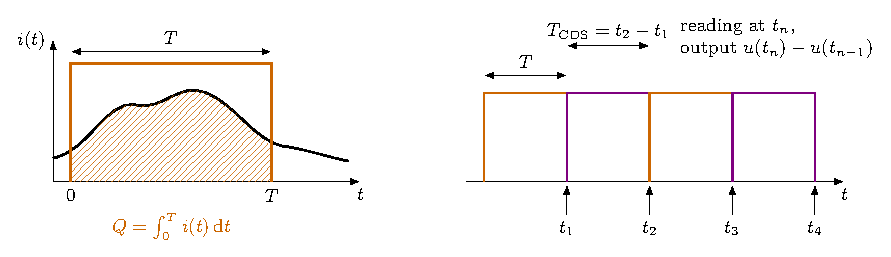
\includegraphics[width=\linewidth]{nausicaa_vh_windows.pdf}
\caption{Left: the gated integrator. The current of one frame is integrated
over a window of length $T$; the shaded area is the charge $Q$. Right: the
frame sequence. Consecutive windows follow each other without gaps, the
output is read at the end of each one, and the measurement is the difference
of consecutive readings, $\Tcds$ apart.}
\label{fig:windows}
\end{figure}
%
The ions of one frame arrive during a window of length $T$
(Fig.~\ref{fig:windows}, left). The amplifier integrates the current over
that window:
%
\begin{equation}
 Q = \int_0^T i(t)\,\dd t .
\end{equation}
%
As a filter acting on the current, this is a convolution with a rectangle of
height 1 and length $T$. Its Fourier transform is
%
\begin{equation}
 H(f) = T\,\sinc(\pi fT)\,e^{-j\pi fT},
 \qquad \sinc x = \frac{\sin x}{x},
\label{eq:sinc}
\end{equation}
%
equivalently $T\,\sinc(\omega T/2)$ with $\omega=2\pi f$. The factor $T$
is the DC gain of the window: a constant current $i$ gives the
charge $iT$. Applied to the noise charge, the same window must be normalised
by $1/T$, because a constant charge on the input gives that charge and not
$T$ times it. The normalised weighting is therefore
%
\begin{equation}
 |W(f)|^2 = \sinc^2(\pi fT).
\label{eq:W1}
\end{equation}
%
Keeping the factor $T$ in both the signal and the noise expression gives the
same ENC, since it cancels in the ratio. The sinc function equals 1 at
$f=0$, has its first zero at $f=1/T$ and decays as $1/f^2$ beyond. Two
consequences follow.
%
\begin{itemize}
\item White noise above $1/T$ is averaged away. With
  $\int_0^\infty\sinc^2(\pi fT)\,\dd f=1/(2T)$, the thermal contribution is
%
  \begin{equation}
   \mathrm{ENC}_t^2 = \frac{\CD^2\,e_t^2}{2T\,e^2}.
  \label{eq:enct}
  \end{equation}
%
  A longer frame gives less thermal noise. For $\CD=\SI{1.25}{pF}$,
  $e_t=\SI{5}{nV/\sqrt{Hz}}$ and $T=\SI{40}{ms}$ this is 0.14 electrons: the
  white part is irrelevant at frame time scales.
\item Flicker noise below $1/T$ is not averaged (Fig.~\ref{fig:spectra},
  left). The flicker contribution is
  $\CD^2A_f\int\sinc^2(\pi fT)\,\dd f/f$, which diverges logarithmically at
  low frequency. It must be cut at the lowest frequency the measurement can
  resolve, $f_l$, which is the inverse of the time between the reference
  level and the measurement. The result is of order
  $\CD^2A_f\,\ln[1/(\pi f_lT)]$. The longer the amplifier runs between
  references, the larger this term.
\end{itemize}
%
The resistor term with the same window is dominated by its low-frequency
end, where the window equals 1 and the spectrum of Eq.~\eqref{eq:qR} rises
as $1/f^2$. The cleaner statement is in the time domain: a white current
noise integrated over $T$ gives a charge variance
%
\begin{equation}
 \boxed{\;\mathrm{ENC}_R^2 = \frac{4kT_{\rm K}}{R_f}\,\frac{T}{2\,e^2}\;}.
\label{eq:encR}
\end{equation}
%
This term grows with the frame length, the opposite of the thermal term. If
the NAUSICAA feedback transistor behaved as a resistor at \SI{300}{K} with
the value implied by its \SI{19.5}{s} decay and $\Cf=\SI{3}{fF}$, about
\SI{6.5}{T\ohm}, a \SI{40}{ms} frame would carry 44 electrons of resistor
noise. The transistor operates in weak inversion and its noise is the SPICE
spectrum reported in \code{csa_design.tex}, which is the number to compare
with. The decisive point is architectural: an amplifier that is reset by a
switch has no $R_f$ and no such term at all.

% ----------------------------------------------------------------------
\section{Correlated double sampling}
\label{sec:cds}
%
The flicker term of Section~\ref{sec:gated} depends on how long the amplifier
runs since its reference. Correlated double sampling removes that
dependence. The measurement is the difference of two samples of the output
taken $\Tcds$ apart (Fig.~\ref{fig:windows}, right),
%
\begin{equation}
 y(t) = x(t) - x(t-\Tcds).
\end{equation}
%
This is a linear filter with impulse response
$h(t)=\delta(t)-\delta(t-\Tcds)$ and transfer function
%
\begin{equation}
 h(f) = 1-e^{-j2\pi f\Tcds}
      = e^{-j\pi f\Tcds}\,2j\,\sin(\pi f\Tcds),
 \qquad
 |h(f)|^2 = 4\sin^2(\pi f\Tcds).
\label{eq:cds}
\end{equation}
%
At low frequency $\sin x\simeq x$ and
%
\begin{equation}
 |h(f)|^2 \simeq 4\pi^2 f^2\Tcds^2 = \omega^2\Tcds^2 ,
 \qquad f\ll 1/\Tcds .
\label{eq:cdslow}
\end{equation}
%
The filter multiplies the spectrum by $f^2$ at low frequency. Three things
disappear.
%
\begin{itemize}
\item A constant offset of the amplifier, $\Voff$, is the same in both
  samples and cancels exactly. It is the $f=0$ component.
\item Slow drifts, with periods longer than $\Tcds$, are strongly attenuated.
\item Flicker noise, whose $1/f$ spectrum would diverge, is multiplied by
  $f^2$ and becomes integrable. The low-frequency cut $f_l$ of
  Section~\ref{sec:gated} is no longer needed.
\end{itemize}
%
Noise above $1/\Tcds$ has twice the mean square after the subtraction,
since the two samples are then independent and the variance of their
difference is the sum of their variances. This is the price
of the subtraction.

In NAUSICAA the reconstruction already forms the difference of consecutive
frame readings, $u(t_n)-u(t_{n-1})$, in the digital domain. That difference
is this filter with $\Tcds=T$.

% ----------------------------------------------------------------------
\section{Total noise with both filters}
\label{sec:total}
%
Applying the window of Eq.~\eqref{eq:W1} and the subtraction of
Eq.~\eqref{eq:cds} in sequence, the weighting function is their product and
%
\begin{equation}
 \mathrm{ENC}^2 = \frac{\CD^2}{e^2}\int_0^\infty
 \sinc^2(\pi fT)\;4\sin^2(\pi f\Tcds)\;
 \left[e_t^2+\frac{A_f}{f}\right]\dd f ,
\label{eq:total}
\end{equation}
%
The integrand has three factors: the sinc falling from 1, the noise profile
falling as $1/f$ then flat, and the subtraction rising as $f^2$ then
oscillating. The product is small at both ends and peaks near $1/T$
(Fig.~\ref{fig:spectra}).
%
\begin{figure}[htbp]\centering
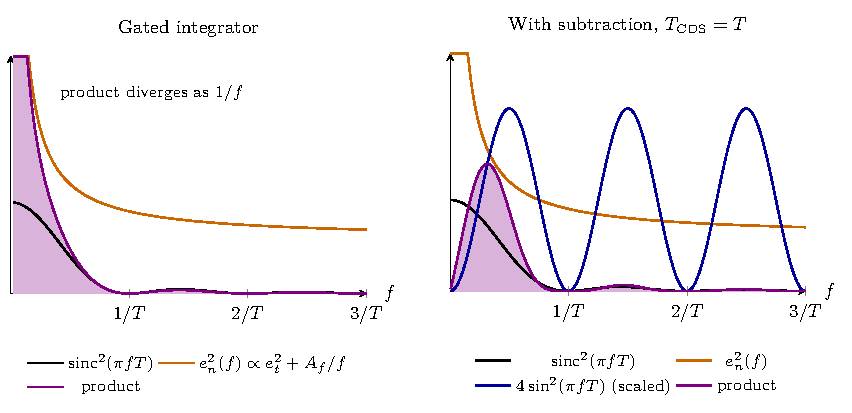
\includegraphics[width=\linewidth]{nausicaa_vh_spectra.pdf}
\caption{The three factors of Eq.~\eqref{eq:total} on a linear frequency
axis, in arbitrary units, for a corner frequency $f_c=0.5/T$. Left: the
gated integrator alone. The window $\sinc^2(\pi fT)$ averages the white
noise above $1/T$, but the product with the $1/f$ profile diverges at low
frequency; its integral depends on the low-frequency cut. Right: with the
subtraction of consecutive frames. The factor $4\sin^2(\pi fT)$ rises as
$f^2$ and cancels the divergence; the product is now concentrated between
$0$ and $1/T$ and its integral is the closed form of
Eq.~\eqref{eq:closed}.}
\label{fig:spectra}
\end{figure}
%

For consecutive frames, $\Tcds=T$, both integrals have closed forms. With
$x=\pi fT$:
%
\begin{align}
 \int_0^\infty \sinc^2(\pi fT)\,4\sin^2(\pi fT)\,\dd f
 &= \frac{4}{\pi T}\int_0^\infty\frac{\sin^4x}{x^2}\,\dd x
  = \frac{4}{\pi T}\cdot\frac{\pi}{4} = \frac{1}{T},
\\
 \int_0^\infty \sinc^2(\pi fT)\,4\sin^2(\pi fT)\,\frac{\dd f}{f}
 &= 4\int_0^\infty\frac{\sin^4x}{x^3}\,\dd x = 4\ln 2 .
\end{align}
%
The two definite integrals are standard~\cite{Gradshteyn2007}. Hence
%
\begin{equation}
 \boxed{\;\mathrm{ENC}^2 = \frac{\CD^2}{e^2}\left[\frac{e_t^2}{T} + 4\ln 2\,A_f\right]\;}.
\label{eq:closed}
\end{equation}
%
The thermal term is twice that of a single window, Eq.~\eqref{eq:enct}, as
expected for a difference of two independent averages. The flicker term is a
pure number times $\CD^2A_f$: it no longer depends on the frame length, nor
on how long the amplifier has been running. With $f_c=\SI{1}{kHz}$ and the
values above it amounts to 2 electrons; the single-window estimate with a
reference \SI{100}{s} earlier would give 3. For a corner at \SI{100}{kHz} the
two numbers are 20 and 32. The subtraction removes the offset completely and
reduces the flicker noise by the logarithm of the time since the last
reference. In words, the largest noise component is strongly reduced; in
numbers, the reduction is that logarithm.

The resistor term, if present, is of the same size with or without the
subtraction: the difference of two integrals of a white current has the
variance of Eq.~\eqref{eq:encR}. This is the reason the reset architecture
is attractive at long frame times.

% ----------------------------------------------------------------------
\section{The two-capacitor architecture}
\label{sec:swap}
%
\begin{figure}[htbp]\centering
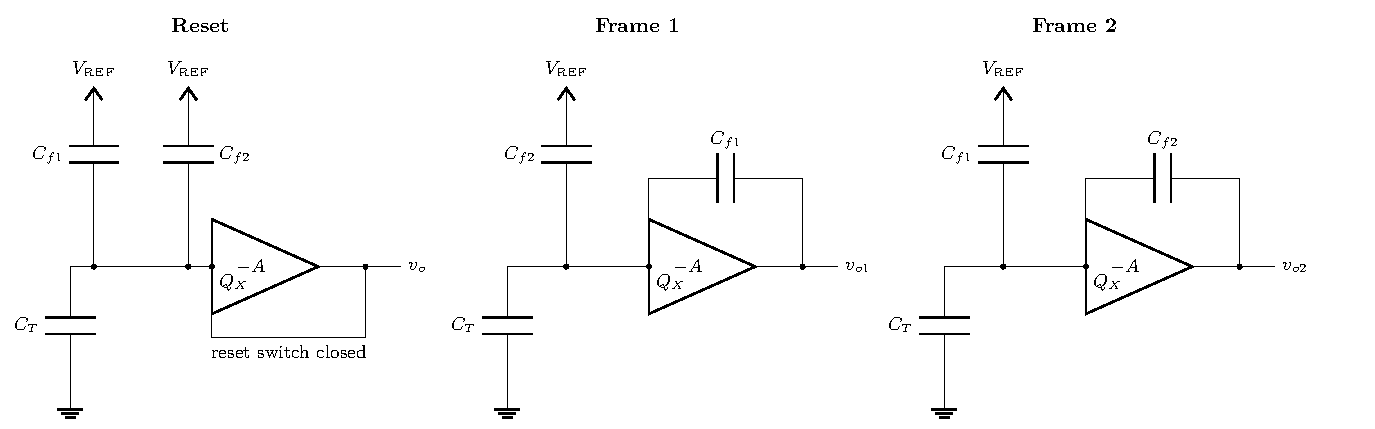
\includegraphics[width=\linewidth]{nausicaa_vh_swap.pdf}
\caption{The two feedback capacitors through one cycle. $C_T$ is the total
capacitance at the input node, $Q_X$ its charge. During reset both capacitors
are connected between the input node and $\Vref$ and the output is shorted to
the input. In frame 1 $C_{f1}$ is the feedback element while $C_{f2}$ stays at
$\Vref$; in frame 2 the roles are exchanged.}
\label{fig:swap}
\end{figure}
%
A circuit can perform the subtraction of Section~\ref{sec:cds} without a
second sample. Two equal capacitors
$C_{f1}=C_{f2}$ alternate between the feedback position and a parking
position at the reference voltage $\Vref$ (Fig.~\ref{fig:swap}). The
amplifier has an offset $\Voff$: it holds its input node at $\Voff$, so the
virtual ground sits at that voltage. The analysis is charge conservation at
the input node, which is isolated except for the signal charge $Q_{i}$ that
arrives during each frame. The charge on $C_T$ is $C_T\Voff$ in every phase
and drops out of every balance below.

%
\paragraph{Reset.} Both capacitors have one plate at the input node, at
$\Voff$, and the other at $\Vref$. The plate at the input node carries
%
\begin{equation}
 Q_{X,R} = -(\Vref-\Voff)(C_{f1}+C_{f2}).
\end{equation}
%

\paragraph{Frame 1.} $C_{f1}$ now connects the input node to the output
$v_{o1}$; $C_{f2}$ stays at $\Vref$. A charge $Q_{i1}$ arrives. The input-node
plates carry
%
\begin{equation}
 Q_{X,S1} = -(\Vref-\Voff)\,C_{f2} + (\Voff-v_{o1})\,C_{f1}.
\end{equation}
%
Conservation, $Q_{X,R}+Q_{i1}=Q_{X,S1}$, gives after cancelling the $C_{f2}$
terms
%
\begin{equation}
 -(\Vref-\Voff)C_{f1}+Q_{i1} = (\Voff-v_{o1})C_{f1}
 \quad\Longrightarrow\quad
 \boxed{\,v_{o1} = \Vref - \frac{Q_{i1}}{C_{f1}}\,}.
\label{eq:vo1}
\end{equation}
%
The offset has cancelled: the two $\Voff C_{f1}$ terms are equal on both
sides. The output is the reference voltage minus the collected charge divided
by the feedback capacitance.

%
\paragraph{Frame 2.} The capacitors exchange roles and $Q_{i2}$ arrives:
%
\begin{equation}
 Q_{X,S2} = -(\Vref-\Voff)\,C_{f1} + (\Voff-v_{o2})\,C_{f2},
 \qquad Q_{X,S1}+Q_{i2}=Q_{X,S2}.
\end{equation}
%
Substituting Eq.~\eqref{eq:vo1} for the $C_{f1}$ term of $Q_{X,S1}$ and
cancelling,
%
\begin{equation}
 \boxed{\,v_{o2} = \Vref - \frac{Q_{i1}+Q_{i2}}{C_{f2}}\,}.
\label{eq:vo2}
\end{equation}
%
Again every $\Voff$ term cancels. Three facts follow from
Eqs.~\eqref{eq:vo1} and \eqref{eq:vo2}.
%
\begin{itemize}
\item Each output is referred to $\Vref$, a clean external voltage, and the
  amplifier offset never appears. This is the subtraction of
  Section~\ref{sec:cds} done by the capacitor swap: the parked capacitor
  carries the reference into the feedback position.
\item The charge accumulates: $v_{o2}$ holds $Q_{i1}+Q_{i2}$, and after $n$
  frames the output holds the sum of all charge since reset. The charge of
  one frame is the difference of consecutive outputs, as in NAUSICAA now, and
  the total charge of a track is read directly.
\item The reset switch deposits a random charge of variance $kT_{\rm K}C$ on
  the capacitors. Because every later output is measured against the same
  reset, this charge cancels in differences, which is the original purpose of
  correlated double sampling in CCDs~\cite{Janesick2001}.
\end{itemize}

% ----------------------------------------------------------------------
\section{What follows for the design}
\label{sec:conclusions}
%
Four design conclusions follow from the two-capacitor architecture. Each has
a reason and a cost.
%
\begin{itemize}
\item \textbf{Offset and flicker cancellation in the analogue domain.}
  Eqs.~\eqref{eq:vo1} and \eqref{eq:vo2} give the subtraction without
  storing and subtracting digital samples. The cost is the switch network at
  the input node, whose charge injection and leakage must be controlled.
\item \textbf{Fewer ADC conversions.} One conversion per frame suffices, since
  the output already holds the accumulated charge. The present NAUSICAA plan
  samples every \SI{100}{\micro s} and averages 50 samples over \SI{5}{ms}
  before differencing; that average is the sinc window of
  Section~\ref{sec:gated} with $T=\SI{5}{ms}$ applied inside the frame.
\item \textbf{A larger feedback capacitance.} Since the charge of a track
  accumulates, the full-scale output must hold the whole track and the
  converter must resolve one frame's charge within it. A larger $\Cf$ lowers
  the voltage per ion and so the range needed; it also lowers the closed-loop
  bandwidth, which Section~\ref{sec:real} shows to be favourable for
  stability. The cost is a smaller signal per ion at the ADC.
\item \textbf{A sigma-delta converter of 16 bits.} With accumulation the
  converter needs range and resolution together: 12 bits are 4096 levels,
  16 bits are 65\,536. A sigma-delta converter averages over its conversion
  time, which is one more sinc window and costs nothing at frame time
  scales.
\end{itemize}

% ----------------------------------------------------------------------
\section{The amplifier: a cascode with degeneration}
\label{sec:cascode}
%
\begin{figure}[htbp]\centering
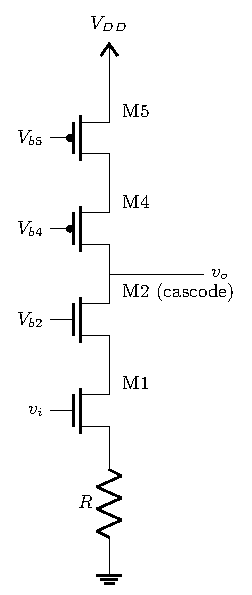
\includegraphics[height=70mm]{nausicaa_vh_cascode.pdf}
\caption{Single-stage amplifier: input transistor M1 with a degeneration
resistor $R$ in its source, cascode M2, and a cascoded PMOS load
M4, M5. The output is the drain node of M2.}
\label{fig:cascode}
\end{figure}
%
A single-stage amplifier suited to this front end is shown in
Fig.~\ref{fig:cascode}. The input transistor M1 converts the input voltage
into a current; the cascode M2 passes that current to a high-impedance output
node; the PMOS pair M4, M5 is the load. A resistor $R$ in the source of M1 is
the new element.

%
\paragraph{Transconductance with degeneration.} Let $v_i$ be the gate voltage
and $i$ the drain current of M1. The source sits at $iR$, so the gate-source
voltage is $v_i-iR$ and $i=g_{m1}(v_i-iR)$. Solving,
%
\begin{equation}
 i = \frac{g_{m1}}{1+g_{m1}R}\,v_i \equiv G_m\,v_i .
\label{eq:Gm}
\end{equation}
%
For $g_{m1}R\gg1$ the transconductance tends to $1/R$: it is then set by a
resistor and no longer by the transistor's operating point, so the stage
stays linear over a wide range of input. A large open-loop gain inside the
feedback loop linearises the closed-loop response in the same way.

%
\paragraph{Gain.} The current $G_mv_i$ flows into the output node, whose
impedance is the parallel combination of the two cascodes. Looking up into
M4, M5 the impedance is about $g_{m4}r_{d4}r_{d5}$; looking down into M2 it is
about $g_{m2}r_{d2}$ times the impedance at the source of M2, which is the
parallel of $r_{d3}$ and the degenerated output of M1, $g_{m1}r_{d1}R$. Here
$r_d$ is the drain-source resistance of each transistor. The open-loop gain
is
%
\begin{equation}
 A = G_m\,Z_o,
 \qquad
 Z_o = \left(g_{m4}r_{d4}r_{d5}\right)\parallel
       \left[g_{m2}r_{d2}\,\big(r_{d3}\parallel g_{m1}r_{d1}R\big)\right].
\end{equation}
%
Each cascode multiplies an output resistance by a factor $g_mr_d$, which is
why a single stage can reach gains of several thousand.

%
\paragraph{Noise.} The resistor adds nothing to the transistor's own noise.
It adds its own: the thermal voltage noise $4kT_{\rm K}R$ of $R$ is in series
with the source of M1, hence in series with the gate-source voltage, and
appears at the input with that full value. Since $e_t^2=4kT_{\rm K}\gamma/g_{m1}$
for the transistor, the resistor adds the same noise as the transistor once
$R\simeq\gamma/g_{m1}$. Degeneration is therefore likely to increase the
noise budget; in current form the added term is $i_n^2=4kT_{\rm K}/R$.

% ----------------------------------------------------------------------
\section{The real amplifier: bandwidth and stability}
\label{sec:real}
%
A real amplifier has finite bandwidth. The simplest model replaces the ideal
gain by a single-pole response
%
\begin{equation}
 A(s) = \frac{A}{1+s/\omega_0},
\end{equation}
%
where $\omega_0$ is the dominant pole of the amplifier. For the stage of
Fig.~\ref{fig:cascode} that pole is formed by the output impedance and the
capacitance at the output node: $\omega_0=1/(Z_oC_o)$, with $C_o$ the sum of
the load capacitance and of $\Cf$ as seen from the output. Inserting $A(s)$ in
Eq.~\eqref{eq:vofull} with $\CD\ll A\Cf$, and writing $Z_f=1/(s\Cf)$ for
the impedance of the feedback capacitor, the ratio of output voltage to input
current is
%
\begin{equation}
 A_{CL}(s) = \frac{Z_f\,A(s)}{1+A(s)}
 = Z_f\,\frac{A}{1+A}\;\frac{1}{1+\dfrac{s}{(1+A)\,\omega_0}} .
\label{eq:acl}
\end{equation}
%
The closed-loop response has a pole at $(1+A)\omega_0$. Feedback extends the
bandwidth by the loop gain. The product
%
\begin{equation}
 \mathrm{GBP} = A\,\omega_0 = G_m Z_o\cdot\frac{1}{Z_oC_o} = \frac{G_m}{C_o}
 \;\simeq\;\frac{g_{m1}}{\Cf}
\label{eq:gbp}
\end{equation}
%
is the gain-bandwidth product and equals the closed-loop bandwidth
(Fig.~\ref{fig:bode}). The last form holds when $\Cf$ dominates $C_o$ and
$R$ is absent.
%
\begin{figure}[htbp]\centering
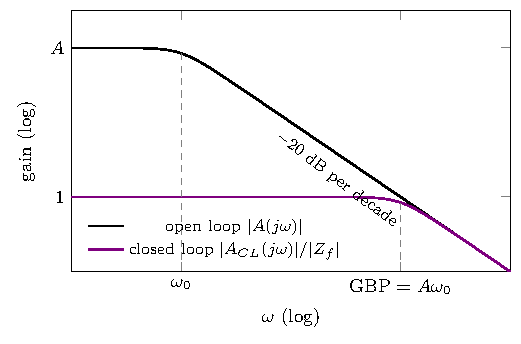
\includegraphics[width=.62\linewidth]{nausicaa_vh_bode.pdf}
\caption{Open-loop gain of the single-pole amplifier and closed-loop gain
of the charge amplifier, normalised to $|Z_f|$, on logarithmic axes
($A=10^4$). The open-loop gain is flat up to $\omega_0$ and falls by a
factor 10 per decade beyond it, crossing unity at the gain-bandwidth product
$A\omega_0$. Feedback trades the gain $A$ for bandwidth: the closed-loop
response is flat up to $(1+A)\omega_0$ and then follows the open-loop
curve.}
\label{fig:bode}
\end{figure} With the pad capacitance included the exact closed-loop pole is
$g_{m1}/(\CD+\Cf)$: the amplifier responds in a time $(\CD+\Cf)/g_{m1}$,
nanoseconds for picofarads and millisiemens.

A design constraint follows from Eq.~\eqref{eq:gbp}. Low
thermal noise requires a large $g_{m1}$; a high charge gain requires a small
$\Cf$; the two together give a very large GBP. With $g_{m1}=\SI{1}{mS}$ and
$\Cf=\SI{3}{fF}$ the ratio is \SI{3e11}{rad/s}. No single-stage amplifier is
that fast, so the second pole of the stage, at the cascode nodes, falls inside
the loop bandwidth and the phase margin is lost. Three remedies exist.
%
\begin{itemize}
\item The degeneration resistor lowers $G_m$ and with it the GBP, at the
  noise cost of Section~\ref{sec:cascode}.
\item A load capacitor $C_L$ at the output lowers $\omega_0$ and sets the
  dominant pole deliberately.
\item A second voltage-gain stage after the integrator lets $\Cf$ be larger
  while the overall sensitivity per ion is preserved; the larger $\Cf$ lowers
  the GBP.
\end{itemize}
%
Each remedy trades bandwidth, which is not needed at frame time scales,
against noise or complexity.

% ----------------------------------------------------------------------
\section{Pad capacitance and input impedance}
\label{sec:cd}
%
Does a pad of \SIrange{1}{5}{pF}, DC coupled to the amplifier, deliver its
charge to the amplifier? The answer is the input impedance of the real
amplifier. From Eq.~\eqref{eq:kcl} the current drawn by
the feedback branch is $s\Cf(1+A(s))v_i$, so
%
\begin{equation}
 Z_{\rm in}(s) = \frac{1}{s\Cf\,[1+A(s)]}
 = \frac{1+s/\omega_0}{s\Cf\,[1+A+s/\omega_0]}.
\label{eq:zin}
\end{equation}
%
Three regimes follow (Fig.~\ref{fig:zin}).
%
\begin{figure}[htbp]\centering
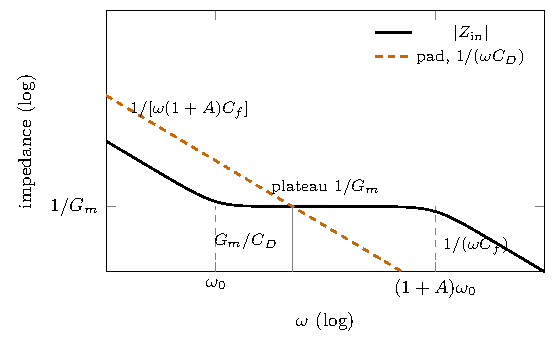
\includegraphics[width=.62\linewidth]{nausicaa_vh_zin.pdf}
\caption{Magnitude of the input impedance of Eq.~\eqref{eq:zin} on
logarithmic axes, for $A=10^4$ and $\CD=400\,\Cf$. Below $\omega_0$ it is
the Miller capacitance $(1+A)\Cf$; between $\omega_0$ and $(1+A)\omega_0$ it
is the plateau $1/G_m$; above, the bare $\Cf$. The dashed line is the
impedance of the pad. The pad delivers its charge to the amplifier where its
impedance lies above $|Z_{\rm in}|$, that is below $\omega=G_m/\CD$.}
\label{fig:zin}
\end{figure}
%
\begin{itemize}
\item Below $\omega_0$: $Z_{\rm in}\simeq1/[s\Cf(1+A)]$, a capacitor of value
  $(1+A)\Cf$: the Miller capacitance of Section~\ref{sec:csa}.
\item Between $\omega_0$ and $(1+A)\omega_0$: the numerator and denominator
  both grow with $s$ and the magnitude is flat,
  $|Z_{\rm in}|\simeq1/(A\Cf\omega_0)=1/G_m$. The input impedance of a
  charge amplifier at these frequencies is the inverse transconductance of
  its input transistor.
\item Above $(1+A)\omega_0$: $Z_{\rm in}\simeq1/(s\Cf)$, the bare feedback
  capacitor, since the amplifier no longer responds.
\end{itemize}
%
The pad delivers its charge to the amplifier when its own impedance
$1/(\omega\CD)$ is much larger than $Z_{\rm in}$ at the frequencies of the
signal. On the plateau the condition reads $\omega\CD\ll G_m$, that is,
$\omega\ll G_m/\CD$. For $\CD=\SI{5}{pF}$ and $G_m=\SI{1}{mS}$ the limit is
\SI{2e8}{rad/s}. Ion signals with \SI{40}{ms} frames are seven orders of
magnitude slower. The pad capacitance therefore does not limit charge
transfer in NAUSICAA. Its effect is on the noise, through
Eq.~\eqref{eq:qn}, and on the closed-loop bandwidth, through
$g_{m1}/(\CD+\Cf)$.

% ----------------------------------------------------------------------
\section{Relation to the present NAUSICAA readout}
\label{sec:nausicaa}
%
Table~\ref{tab:compare} sets the reset architecture of
Section~\ref{sec:swap} beside the amplifier that this repository simulates
and has calibrated.
%
\begin{table}[htbp]\centering\small
\begin{tabular}{@{}p{34mm}p{58mm}p{58mm}@{}}
\toprule
 & Present NAUSICAA circuit & Reset architecture\\
\midrule
Charge removal & Feedback transistor, decay \SI{19.5}{s}, $\Cf=\SI{3}{fF}$ &
Reset switch; no discharge element\\
Reference per frame & Digital difference of consecutive readings; discharge term
$\tau_f^{-1}\int u\,\dd t$ corrected in reconstruction & Analogue: capacitor
swap, output referred to $\Vref$\\
Offset and flicker & Removed by the digital difference & Removed by the swap\\
Discharge-element noise & Present; measured in SPICE & Absent\\
Reset noise & None & $kT_{\rm K}C$, cancelled by the common reset\\
Nonlinearity & Feedback transistor; calibrated nonlinear model with \SI{0.63}{V}
guard & Linear integrator up to the output range; range set by $\Cf$ and the
ADC\\
Conversion & 12 bits every \SI{100}{\micro s}, 50-sample average over \SI{5}{ms}
& One 16-bit sigma-delta conversion per frame\\
Charge per frame & From differences and the discharge correction & From
differences; total charge read directly\\
\bottomrule
\end{tabular}
\caption{The two readout schemes side by side. The present values are those
of \texttt{itaca\_poo.tex} and \texttt{csa\_design.tex}.}
\label{tab:compare}
\end{table}
%

Three points carry over regardless of which circuit is built.
%
\begin{itemize}
\item The frame difference already used in the NAUSICAA reconstruction is the
  filter of Eq.~\eqref{eq:cds}. The closed forms of Eq.~\eqref{eq:closed}
  give the thermal and flicker noise of that reconstruction in terms of
  $\CD$, $e_t$, $A_f$ and $T$. They are an independent check of the bucket
  noise covariance computed from the SPICE spectrum in
  \code{bucket_noise_covariance.jl}.
\item The discharge-element term of Eq.~\eqref{eq:encR} grows with the frame
  length and is untouched by the frame difference. Whether it matters for the
  present circuit is decided by the measured noise spectrum of the feedback
  transistor, which the SPICE model contains. The analytical expression says
  what to look for: a term proportional to $T$.
\item The pad capacitance enters the noise as $\CD^2$ and the bandwidth as
  $\CD/g_{m1}$, and does not limit charge collection. The
  \SI{1.25}{pF} of the calibrated circuit and the \SIrange{1}{5}{pF} range
  of the TopMetal pad lie in the same regime.
\end{itemize}
%
If the two-capacitor architecture is adopted, the itrack stage~2 of the
readout description changes from feedback discharge and digital filtering to
reset, swap and one conversion per frame, and the calibration must be
repeated for the new circuit. The nonlinear model and its guard become
unnecessary; the range limit becomes a reset.

% ----------------------------------------------------------------------
\bibliographystyle{unsrtnat}
\bibliography{references}
\end{document}

